Los resultados del experimento se han recogido en la tabla \cref{tab:results}. Como se puede observar, todas las tareas han implicado más esfuerzo debido a las pruebas unitarias que se han realizado haciendo el uso del marco. Sin embargo, la configuración inicial del proyecto mediante el marco de trabajo ha sido nula, tal y como estaba previsto. De esta tabla cabe destacar que el esfuerzo que nos ha ahorrado el marco de trabajo corresponde a las tareas de Montar el servidor y la integración con el servidor, que han sido un total de 3 horas.

Se han encontrado un total de 20 errores en la implementación sin marco, mientras que el marco nos ha evitado todos los errores. Estos errores han sido encontrados una vez he acabado los dos proyectos. He ido revisando todos los casos de prueba y realizándolos manualmente en el proyecto sin marco. El resultado ha sido que ha habido 20 problemas que, utilizando pruebas unitarias he identificado y resuelto con antelación, mientras que sin realizar estas pruebas se me han pasado por alto. El listado de errores concretos se puede encontrar en la tabla \cref{tab:errors}.

Una vez identificados los erroes, se ha dedicado esfuerzo a solucionarlos y se ha añadido una columna a la tabla \cref{tab:errors} con ese tiempo. El tiempo total ha sido de más de 4 horas. En la figura \cref{fig:results-comparison} se puede apreciar la diferencia del esfuerzo dedicado en el proyecto sin marco de trabajo y el proyecto con marco de trabajo, que casualmente ha sido de 4 horas.

En resumen, por un lado el proyecto sin marco de trabajo nos ha ahorrado 4 horas en total en desarrollo de pruebas unitarias. De las horas dedicadas, 3 han sido evitadas por el marco de trabajo. Es decir, que si hubiésemos realizado el proyecto sin código de calidad, pero utilizando el marco de trabajo, habríamos dedicado 8 horas en total. Por otro lado, se han producido 20 errores desarrollando sin pruebas automáticas, lo cual ha llevado 4 horas y 10 minutos solucionarlos.

% Please add the following required packages to your document preamble:
% \usepackage[table,xcdraw]{xcolor}
% If you use beamer only pass "xcolor=table" option, i.e. \documentclass[xcolor=table]{beamer}
\begin{table}[]
\centering
\caption{Tabla de resultados}
\label{tab:results}
\begin{adjustbox}{width=\columnwidth,center}
\begin{tabular}{llllll}
{\color[HTML]{000000} }                                                & {\color[HTML]{000000} }                         & \multicolumn{2}{l}{{\color[HTML]{000000} \textbf{Sin marco de trabajo}}}                              & \multicolumn{2}{l}{{\color[HTML]{000000} \textbf{Con marco de trabajo}}}                                                      \\
{\color[HTML]{000000} \textbf{Tarea}}                                  & {\color[HTML]{000000} \textbf{Tiempo estimado}} & {\color[HTML]{000000} \textbf{Tiempo empleado}} & {\color[HTML]{000000} \textbf{Errores encontrados}} & {\color[HTML]{000000} \textbf{Tiempo empleado (con marco)}} & {\color[HTML]{000000} \textbf{Errores encontrados (con marco)}} \\
{\color[HTML]{000000} \textbf{Montar el servidor (GraphQL y Express)}} & {\color[HTML]{000000} 1}                        & {\color[HTML]{000000} 1.5}                      & {\color[HTML]{000000} 2}                            & {\color[HTML]{000000} 0}                                    & {\color[HTML]{000000} 0}                                        \\
{\color[HTML]{000000} \textbf{Añadir tarea}}                           & {\color[HTML]{000000} 0.5}                      & {\color[HTML]{000000} 1}                        & {\color[HTML]{000000} 0}                            & {\color[HTML]{000000} 1.5}                                  & {\color[HTML]{000000} 0}                                        \\
{\color[HTML]{000000} \textbf{Eliminar tarea}}                         & {\color[HTML]{000000} 0.5}                      & {\color[HTML]{000000} 0.5}                      & {\color[HTML]{000000} 1}                            & {\color[HTML]{000000} 1}                                    & {\color[HTML]{000000} 0}                                        \\
{\color[HTML]{000000} \textbf{Editar tarea}}                           & {\color[HTML]{000000} 0.5}                      & {\color[HTML]{000000} 0.75}                     & {\color[HTML]{000000} 4}                            & {\color[HTML]{000000} 1.5}                                  & {\color[HTML]{000000} 0}                                        \\
{\color[HTML]{000000} \textbf{Marcar tarea}}                           & {\color[HTML]{000000} 0.25}                     & {\color[HTML]{000000} 0.25}                     & {\color[HTML]{000000} 1}                            & {\color[HTML]{000000} 0.75}                                 & {\color[HTML]{000000} 0}                                        \\
{\color[HTML]{000000} \textbf{Obtener lista de tareas}}                & {\color[HTML]{000000} 0.25}                     & {\color[HTML]{000000} 0.5}                      & {\color[HTML]{000000} 1}                            & {\color[HTML]{000000} 1}                                    & {\color[HTML]{000000} 0}                                        \\
{\color[HTML]{000000} }                                                & {\color[HTML]{000000} }                         & {\color[HTML]{000000} }                         & {\color[HTML]{000000} }                             & {\color[HTML]{000000} }                                     & {\color[HTML]{000000} }                                         \\
{\color[HTML]{000000} \textbf{Montar el cliente (Webpack)}}            & {\color[HTML]{000000} 2}                        & {\color[HTML]{000000} 2}                        & {\color[HTML]{000000} 0}                            & {\color[HTML]{000000} 0}                                    & {\color[HTML]{000000} 0}                                        \\
{\color[HTML]{000000} \textbf{Página de lista de tareas}}              & {\color[HTML]{000000} 0.5}                      & {\color[HTML]{000000} 0.5}                      & {\color[HTML]{000000} 0}                            & {\color[HTML]{000000} 2}                                    & {\color[HTML]{000000} 0}                                        \\
{\color[HTML]{000000} \textbf{Componente de campo de texto}}           & {\color[HTML]{000000} 0.5}                      & {\color[HTML]{000000} 0.25}                     & {\color[HTML]{000000} 1}                            & {\color[HTML]{000000} 0.5}                                  & {\color[HTML]{000000} 0}                                        \\
{\color[HTML]{000000} \textbf{Componente de botón de borrar tarea}}    & {\color[HTML]{000000} 0.25}                     & {\color[HTML]{000000} 0.25}                     & {\color[HTML]{000000} 1}                            & {\color[HTML]{000000} 0.75}                                 & {\color[HTML]{000000} 0}                                        \\
{\color[HTML]{000000} \textbf{Componente de botón de editar tarea}}    & {\color[HTML]{000000} 0.5}                      & {\color[HTML]{000000} 1}                        & {\color[HTML]{000000} 2}                            & {\color[HTML]{000000} 2}                                    & {\color[HTML]{000000} 0}                                        \\
{\color[HTML]{000000} \textbf{Componente de tarea}}                    & {\color[HTML]{000000} 0.25}                     & {\color[HTML]{000000} 0.5}                      & {\color[HTML]{000000} 4}                            & {\color[HTML]{000000} 1.25}                                 & {\color[HTML]{000000} 0}                                        \\
{\color[HTML]{000000} \textbf{Componente de caja de tareas}}           & {\color[HTML]{000000} 0.25}                     & {\color[HTML]{000000} 0.25}                     & {\color[HTML]{000000} 0}                            & {\color[HTML]{000000} 1.5}                                  & {\color[HTML]{000000} 0}                                        \\
{\color[HTML]{000000} \textbf{Componente de botón de añadir tarea}}    & {\color[HTML]{000000} 0.25}                     & {\color[HTML]{000000} 0.25}                     & {\color[HTML]{000000} 1}                            & {\color[HTML]{000000} 1.25}                                 & {\color[HTML]{000000} 0}                                        \\
{\color[HTML]{000000} \textbf{Integración con el servidor}}            & {\color[HTML]{000000} 1}                        & {\color[HTML]{000000} 1.5}                      & {\color[HTML]{000000} 2}                            & {\color[HTML]{000000} 0}                                    & {\color[HTML]{000000} 0}
\end{tabular}
\end{adjustbox}
\end{table}

\begin{table}[]
\centering
\caption{Tabla de errores}
\label{tab:errors}
\begin{adjustbox}{width=\columnwidth,center}
\begin{tabular}{rllr}
\multicolumn{1}{l}{\textbf{ID}} & \textbf{Tarea}                                  & \textbf{Descripción del error}                                                     & \multicolumn{1}{l}{\textbf{Tiempo de resolución (min)}} \\
1                               & \textbf{Montar el servidor (GraphQL y Express)} & El esquema GraphQL se lee con una codificación no soportada                        & 5                                                       \\
2                               & \textbf{Montar el servidor (GraphQL y Express)} & Error de CORS                                                                      & 5                                                       \\
3                               & \textbf{Eliminar tarea}                         & Eliminar tarea que no existe devuelve OK                                           & 15                                                      \\
4                               & \textbf{Editar tarea}                           & Editar tarea que no existe devuelve OK                                             & 15                                                      \\
5                               & \textbf{Editar tarea}                           & Editar una tarea marcada (toggled) quita la marca                                  & 5                                                       \\
6                               & \textbf{Editar tarea}                           & Editar una tarea sin texto devuelve OK                                             & 5                                                       \\
7                               & \textbf{Editar tarea}                           & Editar una tarea que tiene el texto repetido no funciona                           & 10                                                      \\
8                               & \textbf{Marcar tarea}                           & Marcar una tarea con el texto repetido a veces no funciona                         & 10                                                      \\
9                               & \textbf{Obtener lista de tareas}                & Si la lista se acaba de vacíar tras eliminar tarea, devuelve error                 & 30                                                      \\
10                              & \textbf{Componente de campo de texto}           & Si la API devuelve error, muestra ese error en el campo de texto                   & 5                                                       \\
11                              & \textbf{Componente de botón de borrar tarea}    & Borrar una tarea recién reordenada borra una tarea distinta                        & 10                                                      \\
12                              & \textbf{Componente de botón de editar tarea}    & Editar una tarea recién reordenada edita una tarea distinta                        & 10                                                      \\
13                              & \textbf{Componente de botón de editar tarea}    & Editar una tarea sin cambiar el texto envía un vacío a la API                      & 5                                                       \\
14                              & \textbf{Componente de tarea}                    & Reordenar una tarea marcada la desmarca                                            & 15                                                      \\
15                              & \textbf{Componente de tarea}                    & Editar una tarea la cambia de orden                                                & 10                                                      \\
16                              & \textbf{Componente de tarea}                    & Editar una tarea y no ponerle texto genera un error en consola                     & 5                                                       \\
17                              & \textbf{Componente de tarea}                    & Marcar y desmarcar una tarea rápidamente la hace desaparecer                       & 45                                                      \\
18                              & \textbf{Componente de botón de añadir tarea}    & Añadir tarea sin escribir nada en el campo de texto envía una petición al servidor & 5                                                       \\
19                              & \textbf{Integración con el servidor}            & Inconsistencia de la cache de Apollo con respecto a los datos del servidor         & 30                                                      \\
20                              & \textbf{Integración con el servidor}            & Error con el tamaño máximo de carga                                                & 10                                                      \\
\multicolumn{3}{l}{\textbf{Tiempo total (min)}}                                                                                                                        & 250                                                     \\
\multicolumn{3}{l}{\textbf{Tiempo total (horas)}}                                                                                                                      & 4.166666667
\end{tabular}
\end{adjustbox}
\end{table}

\begin{figure}
  \centering
  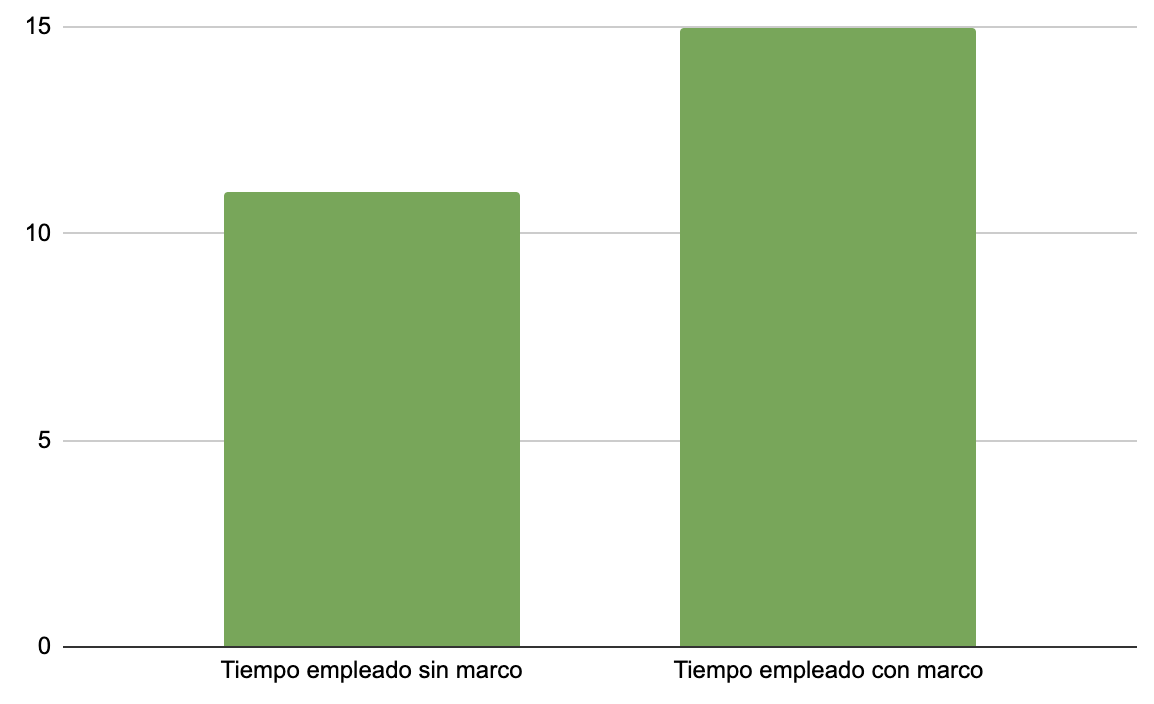
\includegraphics[width=\textwidth]{results-comparison.png}
  \caption{Comparación entre el tiempo dedicado con y sin pruebas}
  \label{fig:results-comparison}
\end{figure}

